% Document  Definition
% Font size: 12pt 
% Document alignment: twoside, possibile singleside

\documentclass[12pt,twoside]{report}

% Import packages 

\usepackage[utf8]{inputenc}
\usepackage{graphicx}
\usepackage[a4paper,width=150mm,right=30mm,left=30mm,top=25mm,bottom=25mm]{geometry}
\usepackage{fancyhdr}
\usepackage{listings}
\usepackage{subcaption}
\usepackage{caption}
\usepackage[table,xcdraw]{xcolor}
\usepackage{comment}
\usepackage{adjustbox}
\usepackage{needspace}
\usepackage[backend=biber]{biblatex}

% Import References Lib

\addbibresource{references.bib}

% Set parameters thesis and packages

\pagestyle{fancy}
\fancyhead{}
\fancyhead[RO,LE]{Thesis Title}
\fancyfoot{}
\fancyfoot[LE,RO]{\thepage}
\fancyfoot[LO,CE]{Chapter \thechapter}
\fancyfoot[CO,RE]{Author Name}
\renewcommand{\headrulewidth}{0.4pt}
\renewcommand{\footrulewidth}{0.4pt}
% Set imges folder paths 
\graphicspath{ {images_support/} {images_thesis/} }
%TITLE
\title{{Thesis Title}\\
	{\large University}\\
	{\label{img:logo_UPC}
	
\includegraphics[scale=0.5]{logo_UPC.jpg}}
}
%AUTHOR
\author{Author}
%DATE
\date{Date}
% start of the document.
\begin{document}
\begin{titlepage}
    \begin{center}
        \large
        \textbf{Master Thesis\\}
        
        \huge
        \vspace{1cm}
        \textbf{Title\\}
        
        \Large
        \vspace{0.5cm}
        Sub Tilte\\
        
        \vspace{1cm}
        
        \textbf{Author\\}
        
        \vspace{1.5cm}
        
        \textbf{Supervised by\\}
        
        Supervisor 1\\
        Supervisor 2\\
        \Large
        \vfill
        Final Project Report for the\\
        Master in ...
        
        \vspace{0.8cm}
        
        
\includegraphics[width=0.4\textwidth]{logo_UPC.jpg}
        
        \vspace{0.8cm}
        Department\\
        University\\
        State, City\\
        Month Year
    \end{center}
\end{titlepage}
% blank page code start
\clearpage\pagestyle{empty}\mbox{}\clearpage
% blank page code end
% front part.
\thispagestyle{plain}
\begin{center}
    \Large
    \textbf{Thesis Title\\}
    \vspace{0.4cm}
    \large
    Thesis Sub Title\\
    \vspace{0.4cm}
    \textbf{Author\\}
    \vspace{0.2cm}
    Supervised by:\\
    \vspace{0.2cm}
    \textbf{Supervisor 1}\\
    Supervisor 1 Department\\
    \textbf{Supervisor 2}\\
    Supervisor 2 Department\\
    \vspace{0.9cm}
    \Huge
    \textbf{Abstract}
\end{center}


Lorem \cite{lorem_web} ipsum dolor sit amet\footnote{amet: Lorem ipsum dolor sit amet.} , consectetur adipiscing elit. Proin pellentesque massa eu lacus vestibulum elementum. Vestibulum nibh neque, blandit a felis nec, sollicitudin lobortis metus. Integer nec ipsum sit amet nibh eleifend maximus. Praesent diam augue, vestibulum a augue ac, egestas aliquet orci. Vivamus eu dui sed nisl fringilla blandit sit amet ac urna. Duis aliquet orci sit amet eleifend cursus. Pellentesque vitae vulputate velit. Curabitur commodo dui at nibh tincidunt, et porttitor nibh tincidunt. Praesent mauris eros, porttitor sed cursus ut, vulputate non purus. Aenean ut nibh quis odio laoreet malesuada volutpat eu elit. Suspendisse vulputate ipsum accumsan nibh ornare ullamcorper. Quisque vitae arcu urna.\par
In et nunc finibus, sodales nibh vitae, vehicula odio. Donec arcu diam, eleifend sed mi ut, congue pellentesque tortor. Ut pretium finibus elit, efficitur elementum ligula euismod nec. In hac habitasse platea dictumst. Vivamus auctor rhoncus magna. Ut venenatis sapien non eros feugiat faucibus. Fusce vel risus eget ante tristique condimentum. Nulla imperdiet rhoncus urna sit amet consectetur.\par
Integer condimentum, arcu non sodales maximus, leo purus viverra lacus, vel tincidunt ligula odio vel urna. Duis ullamcorper orci sed massa sollicitudin, quis auctor elit ullamcorper. Ut eu lacus dignissim, cursus augue in, maximus erat. Morbi pulvinar accumsan est vel placerat. Cras non risus sit amet dolor mattis venenatis eu et ipsum. Sed tincidunt, lectus nec sollicitudin elementum, lectus magna vestibulum tellus, non suscipit diam augue at lorem. Duis venenatis mauris quis ligula scelerisque fermentum. Sed interdum leo et elit efficitur, a scelerisque ante tincidunt. Donec et ultrices ante, tempus vulputate libero. Vivamus molestie blandit enim et sollicitudin. Nunc mauris odio, commodo maximus sollicitudin et, euismod nec tortor. Integer efficitur ipsum dictum sapien luctus efficitur. Sed consectetur tellus id tincidunt porttitor. Pellentesque mattis elit non vestibulum porttitor.\par


\chapter*{Dedication}
% DEDICATION
Lorem ipsum dolor sit amet, consectetur adipiscing elit. Proin pellentesque massa eu lacus vestibulum elementum. Vestibulum nibh neque, blandit a felis nec, sollicitudin lobortis metus. Integer nec ipsum sit amet nibh eleifend maximus. Praesent diam augue, vestibulum a augue ac, egestas aliquet orci. Vivamus eu dui sed nisl fringilla blandit sit amet ac urna. Duis aliquet orci sit amet eleifend cursus. Pellentesque vitae vulputate velit. Curabitur commodo dui at nibh tincidunt, et porttitor nibh tincidunt. Praesent mauris eros, porttitor sed cursus ut, vulputate non purus. Aenean ut nibh quis odio laoreet malesuada volutpat eu elit. Suspendisse vulputate ipsum accumsan nibh ornare ullamcorper. Quisque vitae arcu urna.

\chapter*{Acknowledgements}
% ACKNOWLEDGEMENTS
Lorem ipsum dolor sit amet, consectetur adipiscing elit. Proin pellentesque massa eu lacus vestibulum elementum. Vestibulum nibh neque, blandit a felis nec, sollicitudin lobortis metus. Integer nec ipsum sit amet nibh eleifend maximus. Praesent diam augue, vestibulum a augue ac, egestas aliquet orci. Vivamus eu dui sed nisl fringilla blandit sit amet ac urna. Duis aliquet orci sit amet eleifend cursus. Pellentesque vitae vulputate velit. Curabitur commodo dui at nibh tincidunt, et porttitor nibh tincidunt. Praesent mauris eros, porttitor sed cursus ut, vulputate non purus. Aenean ut nibh quis odio laoreet malesuada volutpat eu elit. Suspendisse vulputate ipsum accumsan nibh ornare ullamcorper. Quisque vitae arcu urna.\par

In et nunc finibus, sodales nibh vitae, vehicula odio. Donec arcu diam, eleifend sed mi ut, congue pellentesque tortor. Ut pretium finibus elit, efficitur elementum ligula euismod nec. In hac habitasse platea dictumst. Vivamus auctor rhoncus magna. Ut venenatis sapien non eros feugiat faucibus. Fusce vel risus eget ante tristique condimentum. Nulla imperdiet rhoncus urna sit amet consectetur.\par


% table of contents with the import of the differents external chapters so its more readable the whole document.
\tableofcontents
% blank page code start
\clearpage\pagestyle{empty}\mbox{}\clearpage
% blank page code end
\listoffigures
% blank page code start
\clearpage\pagestyle{empty}\mbox{}\clearpage
% blank page code end
\listoftables
% blank page code start
\clearpage\pagestyle{empty}\mbox{}\clearpage
% blank page code end
\chapter*{List of Contributions}
\begin{itemize}
  \item  Contribution 1;
  \item  Contribution 2;
  \item  Contribution 3.
\end{itemize}
% blank page code start
\clearpage\pagestyle{empty}\mbox{}\clearpage
% blank page code end
\chapter{Introduction, Motivations and Goals}
\graphicspath{ {images_thesis/} }
\section{Lorem ipsum}
Lorem\cite{lorem_article} ipsum dolor sit amet, consectetur adipiscing elit. Proin pellentesque massa eu lacus vestibulum elementum. Vestibulum nibh neque, blandit a felis nec, sollicitudin lobortis metus. Integer nec ipsum sit amet nibh eleifend maximus. Praesent diam augue, vestibulum a augue ac, egestas aliquet orci. Vivamus eu dui sed nisl fringilla blandit sit amet ac urna. Duis aliquet orci sit amet eleifend cursus. Pellentesque vitae vulputate velit. Curabitur commodo dui at nibh tincidunt, et porttitor nibh tincidunt. Praesent mauris eros, porttitor sed cursus ut, vulputate non purus. Aenean ut nibh quis odio laoreet malesuada volutpat eu elit. Suspendisse vulputate ipsum accumsan nibh ornare ullamcorper. Quisque vitae arcu urna.
\section{In et}
In et nunc finibus, sodales nibh vitae, vehicula odio. Donec arcu diam, eleifend sed mi ut, congue pellentesque tortor. Ut pretium finibus elit, efficitur elementum ligula euismod nec. In hac habitasse platea dictumst. Vivamus auctor rhoncus magna. Ut venenatis sapien non eros feugiat faucibus. Fusce vel risus eget ante tristique condimentum. Nulla imperdiet rhoncus urna sit amet consectetur.
\subsection{Integer}
Integer condimentum, arcu non sodales maximus, leo purus viverra lacus, vel tincidunt ligula odio vel urna. Duis ullamcorper orci sed massa sollicitudin, quis auctor elit ullamcorper. Ut eu lacus dignissim, cursus augue in, maximus erat. Morbi pulvinar accumsan est vel placerat. Cras non risus sit amet dolor mattis venenatis eu et ipsum. Sed tincidunt, lectus nec sollicitudin elementum, lectus magna vestibulum tellus, non suscipit diam augue at lorem. Duis venenatis mauris quis ligula scelerisque fermentum. Sed interdum leo et elit efficitur, a scelerisque ante tincidunt. Donec et ultrices ante, tempus vulputate libero. Vivamus molestie blandit enim et sollicitudin. Nunc mauris odio, commodo maximus sollicitudin et, euismod nec tortor. Integer efficitur ipsum dictum sapien luctus efficitur. Sed consectetur tellus id tincidunt porttitor. Pellentesque mattis elit non vestibulum porttitor.
\subsection{Phasellus}
Phasellus orci massa, tempor eu turpis ac, sollicitudin laoreet risus. Mauris pretium interdum justo, pretium scelerisque urna laoreet cursus. Maecenas semper nisl ultrices felis sollicitudin fringilla. Sed vitae diam malesuada, lacinia orci non, blandit erat. In feugiat consequat maximus. Praesent non venenatis est. Cras finibus auctor risus at feugiat. Vestibulum mi massa, pharetra id ullamcorper sit amet, eleifend a purus. Etiam feugiat consectetur elit. In semper purus sit amet tempor rutrum. Donec sit amet enim sit amet sem tempus malesuada. Mauris quam nulla, tempus sed nunc pharetra, sagittis dignissim risus. Curabitur non erat massa. Morbi tincidunt libero ac mattis viverra. Integer ut leo nec odio facilisis blandit id nec libero. Nulla facilisi.
\section{Morbi}
Morbi ac varius enim, ac lobortis odio. Nullam venenatis, erat in faucibus vestibulum, magna dolor faucibus sapien, ac iaculis tellus urna ut purus. Pellentesque finibus urna eget maximus cursus. Aenean mollis ante nec dolor iaculis, ac malesuada enim ultrices. Aenean vulputate felis sapien, quis rhoncus odio dictum vitae. Proin quis rhoncus velit, et porttitor sem. Pellentesque habitant morbi tristique senectus et netus et malesuada fames ac turpis egestas. Mauris vehicula, arcu tempus scelerisque ultricies, nisl ligula gravida nisl, et dapibus risus leo sit amet odio. Maecenas pellentesque ante eu dolor faucibus suscipit. Vivamus quis semper lectus, vitae interdum velit. Quisque sapien sem, placerat et tempor id, feugiat ut nisi. Nunc at imperdiet mauris, id varius ipsum.


\subsection{Images}

Morbi \ref{fig:template_cat} ac varius enim, ac lobortis odio. Nullam venenatis, erat in faucibus vestibulum, magna dolor faucibus sapien, ac iaculis tellus urna ut purus. Pellentesque finibus urna eget maximus cursus. Aenean mollis ante nec dolor iaculis, ac malesuada enim ultrices. Aenean vulputate felis sapien, quis rhoncus odio dictum vitae.

\begin{figure}[h!]
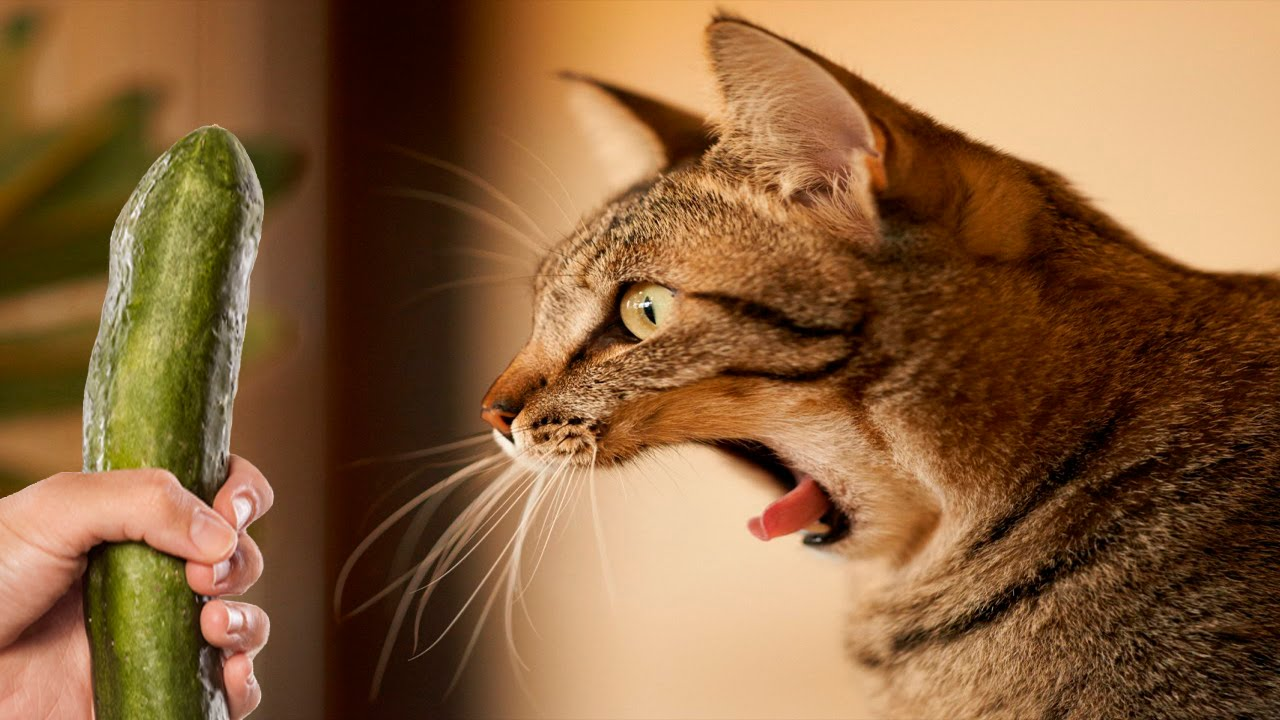
\includegraphics[scale=0.3]{lorem_image.png} 
\centering
\caption{Morbi ac varius enim, ac lobortis odio. Nullam venenatis, erat in faucibus vestibulum, magna dolor faucibus sapien, ac iaculis tellus urna ut purus. Pellentesque finibus urna eget maximus cursus. Aenean mollis ante nec dolor iaculis, ac malesuada enim ultrices. Aenean vulputate felis sapien, quis rhoncus odio dictum vitae.}
\label{fig:template_cat}
\end{figure}

\subsection{Tables}

Morbi \ref{tab:template_table} ac varius enim, ac lobortis odio. Nullam venenatis, erat in faucibus vestibulum, magna dolor faucibus sapien, ac iaculis tellus urna ut purus. Pellentesque finibus urna eget maximus cursus. Aenean mollis ante nec dolor iaculis, ac malesuada enim ultrices. Aenean vulputate felis sapien, quis rhoncus odio dictum vitae.

\begin{table}[h!]
\centering
\begin{tabular}{|c|c|c|c|}
\hline
\textbf{Team name}      & \textbf{Entry description}                                                                                                & \textbf{\begin{tabular}[c]{@{}c@{}}Number of\\  object \\ categories won\end{tabular}} & \textbf{mAP}                    \\ \hline
\textbf{NUIST}          & \begin{tabular}[c]{@{}c@{}}cascaded region regression \\ + tracking\end{tabular}                                          & 10                                                                                     & {\color[HTML]{FE0000} 0.808292} \\ \hline
\textbf{NUIST}          & \begin{tabular}[c]{@{}c@{}}cascaded region regression \\  + tracking\end{tabular}                                         & 10                                                                                     & 0.803154                        \\ \hline
\textbf{CUVideo}        & \begin{tabular}[c]{@{}c@{}}4-model ensemble with\\ Multi-Context Suppression and\\ Motion-Guided Propagation\end{tabular} & 9                                                                                      & 0.767981                        \\ \hline
\textbf{Trimps-Soushen} & Ensemble 2                                                                                                                & 1                                                                                      & 0.709651                        \\ \hline
\end{tabular}
\caption{Morbi ac varius enim, ac lobortis odio. Nullam venenatis, erat in faucibus vestibulum, magna dolor faucibus sapien, ac iaculis tellus urna ut purus. Pellentesque finibus urna eget maximus cursus. Aenean mollis ante nec dolor iaculis, ac malesuada enim ultrices. Aenean vulputate felis sapien, quis rhoncus odio dictum vitae.}
\label{tab:template_table}
\end{table}
% blank page code start
\clearpage\pagestyle{empty}\mbox{}\clearpage
% blank page code end
\chapter{State of the Art}
\input{chapters/4_stateoftheart}
\chapter{Methodology}
\input{chapters/5_methodology}
\chapter{Development of the Work}
\input{chapters/6_development}
\chapter{Evaluation of the Work}
\input{chapters/7_evaluation}
\chapter{Conclusion}
\graphicspath{ {images_thesis/} }
\section{Lorem ipsum}
Lorem ipsum dolor sit amet, consectetur adipiscing elit. Proin pellentesque massa eu lacus vestibulum elementum. Vestibulum nibh neque, blandit a felis nec, sollicitudin lobortis metus. Integer nec ipsum sit amet nibh eleifend maximus. Praesent diam augue, vestibulum a augue ac, egestas aliquet orci. Vivamus eu dui sed nisl fringilla blandit sit amet ac urna. Duis aliquet orci sit amet eleifend cursus. Pellentesque vitae vulputate velit. Curabitur commodo dui at nibh tincidunt, et porttitor nibh tincidunt. Praesent mauris eros, porttitor sed cursus ut, vulputate non purus. Aenean ut nibh quis odio laoreet malesuada volutpat eu elit. Suspendisse vulputate ipsum accumsan nibh ornare ullamcorper. Quisque vitae arcu urna.
\section{In et}
In et nunc finibus, sodales nibh vitae, vehicula odio. Donec arcu diam, eleifend sed mi ut, congue pellentesque tortor. Ut pretium finibus elit, efficitur elementum ligula euismod nec. In hac habitasse platea dictumst. Vivamus auctor rhoncus magna. Ut venenatis sapien non eros feugiat faucibus. Fusce vel risus eget ante tristique condimentum. Nulla imperdiet rhoncus urna sit amet consectetur.
\subsection{Integer}
Integer condimentum, arcu non sodales maximus, leo purus viverra lacus, vel tincidunt ligula odio vel urna. Duis ullamcorper orci sed massa sollicitudin, quis auctor elit ullamcorper. Ut eu lacus dignissim, cursus augue in, maximus erat. Morbi pulvinar accumsan est vel placerat. Cras non risus sit amet dolor mattis venenatis eu et ipsum. Sed tincidunt, lectus nec sollicitudin elementum, lectus magna vestibulum tellus, non suscipit diam augue at lorem. Duis venenatis mauris quis ligula scelerisque fermentum. Sed interdum leo et elit efficitur, a scelerisque ante tincidunt. Donec et ultrices ante, tempus vulputate libero. Vivamus molestie blandit enim et sollicitudin. Nunc mauris odio, commodo maximus sollicitudin et, euismod nec tortor. Integer efficitur ipsum dictum sapien luctus efficitur. Sed consectetur tellus id tincidunt porttitor. Pellentesque mattis elit non vestibulum porttitor.
\subsection{Phasellus}
Phasellus orci massa, tempor eu turpis ac, sollicitudin laoreet risus. Mauris pretium interdum justo, pretium scelerisque urna laoreet cursus. Maecenas semper nisl ultrices felis sollicitudin fringilla. Sed vitae diam malesuada, lacinia orci non, blandit erat. In feugiat consequat maximus. Praesent non venenatis est. Cras finibus auctor risus at feugiat. Vestibulum mi massa, pharetra id ullamcorper sit amet, eleifend a purus. Etiam feugiat consectetur elit. In semper purus sit amet tempor rutrum. Donec sit amet enim sit amet sem tempus malesuada. Mauris quam nulla, tempus sed nunc pharetra, sagittis dignissim risus. Curabitur non erat massa. Morbi tincidunt libero ac mattis viverra. Integer ut leo nec odio facilisis blandit id nec libero. Nulla facilisi.
\section{Morbi}
Morbi ac varius enim, ac lobortis odio. Nullam venenatis, erat in faucibus vestibulum, magna dolor faucibus sapien, ac iaculis tellus urna ut purus. Pellentesque finibus urna eget maximus cursus. Aenean mollis ante nec dolor iaculis, ac malesuada enim ultrices. Aenean vulputate felis sapien, quis rhoncus odio dictum vitae. Proin quis rhoncus velit, et porttitor sem. Pellentesque habitant morbi tristique senectus et netus et malesuada fames ac turpis egestas. Mauris vehicula, arcu tempus scelerisque ultricies, nisl ligula gravida nisl, et dapibus risus leo sit amet odio. Maecenas pellentesque ante eu dolor faucibus suscipit. Vivamus quis semper lectus, vitae interdum velit. Quisque sapien sem, placerat et tempor id, feugiat ut nisi. Nunc at imperdiet mauris, id varius ipsum.


\subsection{Images}

Morbi \ref{fig:template_cat_c} ac varius enim, ac lobortis odio. Nullam venenatis, erat in faucibus vestibulum, magna dolor faucibus sapien, ac iaculis tellus urna ut purus. Pellentesque finibus urna eget maximus cursus. Aenean mollis ante nec dolor iaculis, ac malesuada enim ultrices. Aenean vulputate felis sapien, quis rhoncus odio dictum vitae.

\begin{figure}[h!]
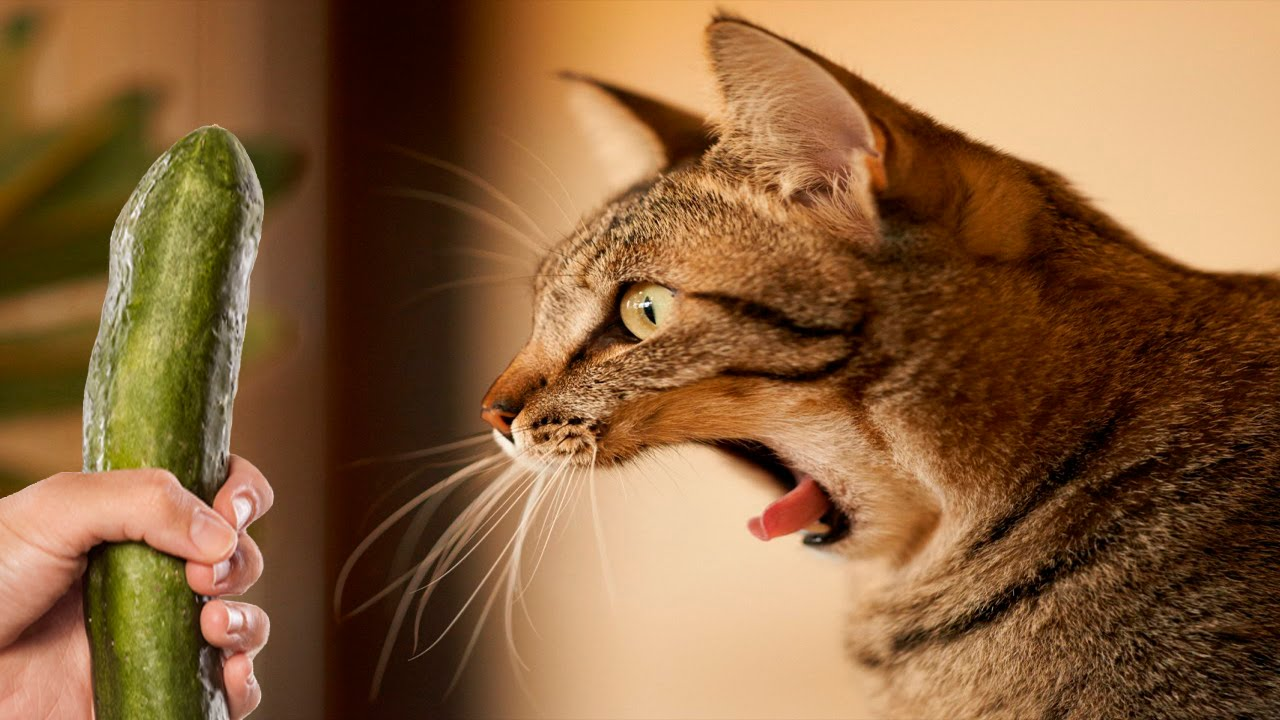
\includegraphics[scale=0.3]{lorem_image.png} 
\centering
\caption{Morbi ac varius enim, ac lobortis odio. Nullam venenatis, erat in faucibus vestibulum, magna dolor faucibus sapien, ac iaculis tellus urna ut purus. Pellentesque finibus urna eget maximus cursus. Aenean mollis ante nec dolor iaculis, ac malesuada enim ultrices. Aenean vulputate felis sapien, quis rhoncus odio dictum vitae.}
\label{fig:template_cat_c}
\end{figure}

\subsection{Tables}

Morbi \ref{tab:template_table_c} ac varius enim, ac lobortis odio. Nullam venenatis, erat in faucibus vestibulum, magna dolor faucibus sapien, ac iaculis tellus urna ut purus. Pellentesque finibus urna eget maximus cursus. Aenean mollis ante nec dolor iaculis, ac malesuada enim ultrices. Aenean vulputate felis sapien, quis rhoncus odio dictum vitae.

\begin{table}[h!]
\centering
\begin{tabular}{|c|c|c|c|}
\hline
\textbf{Team name}      & \textbf{Entry description}                                                                                                & \textbf{\begin{tabular}[c]{@{}c@{}}Number of\\  object \\ categories won\end{tabular}} & \textbf{mAP}                    \\ \hline
\textbf{NUIST}          & \begin{tabular}[c]{@{}c@{}}cascaded region regression \\ + tracking\end{tabular}                                          & 10                                                                                     & {\color[HTML]{FE0000} 0.808292} \\ \hline
\textbf{NUIST}          & \begin{tabular}[c]{@{}c@{}}cascaded region regression \\  + tracking\end{tabular}                                         & 10                                                                                     & 0.803154                        \\ \hline
\textbf{CUVideo}        & \begin{tabular}[c]{@{}c@{}}4-model ensemble with\\ Multi-Context Suppression and\\ Motion-Guided Propagation\end{tabular} & 9                                                                                      & 0.767981                        \\ \hline
\textbf{Trimps-Soushen} & Ensemble 2                                                                                                                & 1                                                                                      & 0.709651                        \\ \hline
\end{tabular}
\caption{Morbi ac varius enim, ac lobortis odio. Nullam venenatis, erat in faucibus vestibulum, magna dolor faucibus sapien, ac iaculis tellus urna ut purus. Pellentesque finibus urna eget maximus cursus. Aenean mollis ante nec dolor iaculis, ac malesuada enim ultrices. Aenean vulputate felis sapien, quis rhoncus odio dictum vitae.}
\label{tab:template_table_c}
\end{table}
% appendix declaration.
\appendix
\chapter{Appendix}
\graphicspath{ {images_thesis/} }
\section{Lorem ipsum}
Lorem ipsum dolor sit amet, consectetur adipiscing elit. Proin pellentesque massa eu lacus vestibulum elementum. Vestibulum nibh neque, blandit a felis nec, sollicitudin lobortis metus. Integer nec ipsum sit amet nibh eleifend maximus. Praesent diam augue, vestibulum a augue ac, egestas aliquet orci. Vivamus eu dui sed nisl fringilla blandit sit amet ac urna. Duis aliquet orci sit amet eleifend cursus. Pellentesque vitae vulputate velit. Curabitur commodo dui at nibh tincidunt, et porttitor nibh tincidunt. Praesent mauris eros, porttitor sed cursus ut, vulputate non purus. Aenean ut nibh quis odio laoreet malesuada volutpat eu elit. Suspendisse vulputate ipsum accumsan nibh ornare ullamcorper. Quisque vitae arcu urna.
\section{In et}
In et nunc finibus, sodales nibh vitae, vehicula odio. Donec arcu diam, eleifend sed mi ut, congue pellentesque tortor. Ut pretium finibus elit, efficitur elementum ligula euismod nec. In hac habitasse platea dictumst. Vivamus auctor rhoncus magna. Ut venenatis sapien non eros feugiat faucibus. Fusce vel risus eget ante tristique condimentum. Nulla imperdiet rhoncus urna sit amet consectetur.
\subsection{Integer}
Integer condimentum, arcu non sodales maximus, leo purus viverra lacus, vel tincidunt ligula odio vel urna. Duis ullamcorper orci sed massa sollicitudin, quis auctor elit ullamcorper. Ut eu lacus dignissim, cursus augue in, maximus erat. Morbi pulvinar accumsan est vel placerat. Cras non risus sit amet dolor mattis venenatis eu et ipsum. Sed tincidunt, lectus nec sollicitudin elementum, lectus magna vestibulum tellus, non suscipit diam augue at lorem. Duis venenatis mauris quis ligula scelerisque fermentum. Sed interdum leo et elit efficitur, a scelerisque ante tincidunt. Donec et ultrices ante, tempus vulputate libero. Vivamus molestie blandit enim et sollicitudin. Nunc mauris odio, commodo maximus sollicitudin et, euismod nec tortor. Integer efficitur ipsum dictum sapien luctus efficitur. Sed consectetur tellus id tincidunt porttitor. Pellentesque mattis elit non vestibulum porttitor.
\subsection{Phasellus}
Phasellus orci massa, tempor eu turpis ac, sollicitudin laoreet risus. Mauris pretium interdum justo, pretium scelerisque urna laoreet cursus. Maecenas semper nisl ultrices felis sollicitudin fringilla. Sed vitae diam malesuada, lacinia orci non, blandit erat. In feugiat consequat maximus. Praesent non venenatis est. Cras finibus auctor risus at feugiat. Vestibulum mi massa, pharetra id ullamcorper sit amet, eleifend a purus. Etiam feugiat consectetur elit. In semper purus sit amet tempor rutrum. Donec sit amet enim sit amet sem tempus malesuada. Mauris quam nulla, tempus sed nunc pharetra, sagittis dignissim risus. Curabitur non erat massa. Morbi tincidunt libero ac mattis viverra. Integer ut leo nec odio facilisis blandit id nec libero. Nulla facilisi.
\section{Morbi}
Morbi ac varius enim, ac lobortis odio. Nullam venenatis, erat in faucibus vestibulum, magna dolor faucibus sapien, ac iaculis tellus urna ut purus. Pellentesque finibus urna eget maximus cursus. Aenean mollis ante nec dolor iaculis, ac malesuada enim ultrices. Aenean vulputate felis sapien, quis rhoncus odio dictum vitae. Proin quis rhoncus velit, et porttitor sem. Pellentesque habitant morbi tristique senectus et netus et malesuada fames ac turpis egestas. Mauris vehicula, arcu tempus scelerisque ultricies, nisl ligula gravida nisl, et dapibus risus leo sit amet odio. Maecenas pellentesque ante eu dolor faucibus suscipit. Vivamus quis semper lectus, vitae interdum velit. Quisque sapien sem, placerat et tempor id, feugiat ut nisi. Nunc at imperdiet mauris, id varius ipsum.


\subsection{Images}

Morbi \ref{fig:template_cat_a} ac varius enim, ac lobortis odio. Nullam venenatis, erat in faucibus vestibulum, magna dolor faucibus sapien, ac iaculis tellus urna ut purus. Pellentesque finibus urna eget maximus cursus. Aenean mollis ante nec dolor iaculis, ac malesuada enim ultrices. Aenean vulputate felis sapien, quis rhoncus odio dictum vitae.

\begin{figure}[h!]
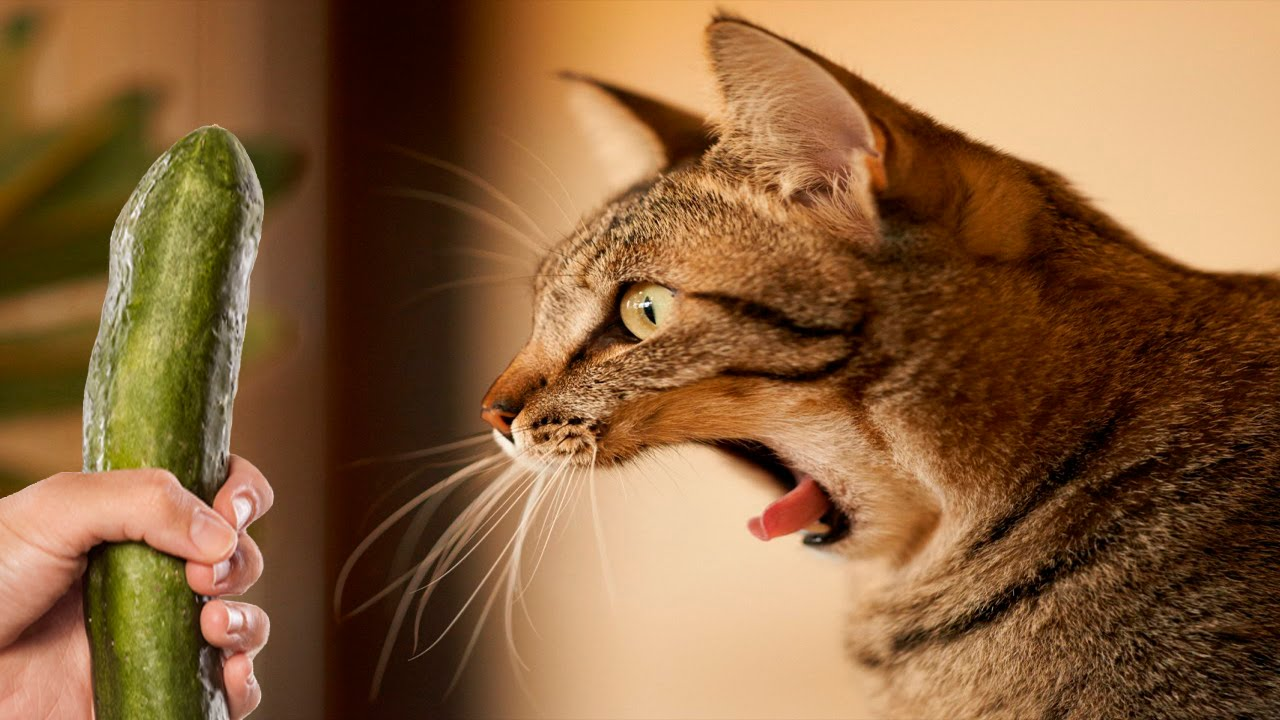
\includegraphics[scale=0.3]{lorem_image.png} 
\centering
\caption{Morbi ac varius enim, ac lobortis odio. Nullam venenatis, erat in faucibus vestibulum, magna dolor faucibus sapien, ac iaculis tellus urna ut purus. Pellentesque finibus urna eget maximus cursus. Aenean mollis ante nec dolor iaculis, ac malesuada enim ultrices. Aenean vulputate felis sapien, quis rhoncus odio dictum vitae.}
\label{fig:template_cat_a}
\end{figure}

\subsection{Tables}

Morbi \ref{tab:template_table_a} ac varius enim, ac lobortis odio. Nullam venenatis, erat in faucibus vestibulum, magna dolor faucibus sapien, ac iaculis tellus urna ut purus. Pellentesque finibus urna eget maximus cursus. Aenean mollis ante nec dolor iaculis, ac malesuada enim ultrices. Aenean vulputate felis sapien, quis rhoncus odio dictum vitae.

\begin{table}[h!]
\centering
\begin{tabular}{|c|c|c|c|}
\hline
\textbf{Team name}      & \textbf{Entry description}                                                                                                & \textbf{\begin{tabular}[c]{@{}c@{}}Number of\\  object \\ categories won\end{tabular}} & \textbf{mAP}                    \\ \hline
\textbf{NUIST}          & \begin{tabular}[c]{@{}c@{}}cascaded region regression \\ + tracking\end{tabular}                                          & 10                                                                                     & {\color[HTML]{FE0000} 0.808292} \\ \hline
\textbf{NUIST}          & \begin{tabular}[c]{@{}c@{}}cascaded region regression \\  + tracking\end{tabular}                                         & 10                                                                                     & 0.803154                        \\ \hline
\textbf{CUVideo}        & \begin{tabular}[c]{@{}c@{}}4-model ensemble with\\ Multi-Context Suppression and\\ Motion-Guided Propagation\end{tabular} & 9                                                                                      & 0.767981                        \\ \hline
\textbf{Trimps-Soushen} & Ensemble 2                                                                                                                & 1                                                                                      & 0.709651                        \\ \hline
\end{tabular}
\caption{Morbi ac varius enim, ac lobortis odio. Nullam venenatis, erat in faucibus vestibulum, magna dolor faucibus sapien, ac iaculis tellus urna ut purus. Pellentesque finibus urna eget maximus cursus. Aenean mollis ante nec dolor iaculis, ac malesuada enim ultrices. Aenean vulputate felis sapien, quis rhoncus odio dictum vitae.}
\label{tab:template_table_a}
\end{table}
\printbibliography 

\end{document}